%\documentclass[handout]{beamer} 
\documentclass[t,12pt,numbers,fleqn]{beamer}
%\documentclass[ignorenonframetext]{beamer}

\newif\ifquestions
%\questionstrue
\questionsfalse

\usepackage{pgfpages} 
\usepackage{hyperref}
\hypersetup{colorlinks=true,
    linkcolor=blue,
    citecolor=blue,
    filecolor=blue,
    urlcolor=blue,
    unicode=false}
\urlstyle{same}

\usepackage{booktabs}
\usepackage{hhline}
\usepackage{multirow}
\usepackage{multicol}
\usepackage{array}

\usepackage{tikz}
\usetikzlibrary{positioning}

%\usepackage{natbib} %doesn't seem to work with beamer
\bibliographystyle{plain}
%\setcitestyle{authoryear}

%\usetheme{Iimenau}

\useoutertheme{split} %so the footline can be seen, without needing pgfpages

%\pgfpagesuselayout{resize to}[letterpaper,border shrink=5mm,landscape]  %if this is uncommented, the hyperref links do not work

\mode<presentation>{}

\input{../def-beamer}

\newcommand{\topic}{02 Getting Started}

%Title page information for 1D04 lectures slides

% Define year specific parameters - used in title page and footer

\newcommand{\season}{Fall} %use to switch between Winter and Fall
\newcommand{\instructor}{Dr.~Spencer Smith} %use to switch instructor
\newcommand{\instructSmall}{Dr.~Smith}
\newcommand{\yr}{2019}
\newcommand{\courseCode}{CAS 741, CES 741}
\newcommand{\courseTitle}{Development of Scientific Computing Software}

%\setbeamerfont{structure}{series=\bfseries}
%\usefonttheme[stillsansseriftext,stillsansserifmath]{serif}
\setbeamertemplate{navigation symbols}{} 
\setbeamertemplate{itemize item}[ball]

\title{
  {\normalsize \bf 
    \borange{\courseCode~(\courseTitle)\\ \season~\yr}}\\[2ex]
  {\Large \bf \topic}}

\author[Smith]{\instructor}

\institute{
  Faculty of Engineering,
  McMaster University}

\date{
\today
%January 2011\\
\bc
  \includegraphics[scale = 0.2, keepaspectratio]
  {../mcmaster-logo-full-color.jpg}
\ec
}

\renewcommand{\borange}[1] %orange is too hard to read
{
   \bred{#1}
}

\begin{document}

%\nobibliography{../../ReferenceMaterial/References}

\input{../footline}

%%%%%%%%%%%%%%%%%%%%%%%%%%%%%%%%%%%%%%%%%%%%%%%%%%

\begin{frame}
\frametitle{Getting Started}

\bi
\item Administrative details
\item Any more introductions?
\item Project choices
\item Software tools
\item Questions on suggested reading?
\item Software Engineering for Scientific Computing literature
\ei

\end{frame}

%%%%%%%%%%%%%%%%%%%%%%%%%%%%%%%%%%%%%%%%%%%%%%%%%%

\begin{frame}
\frametitle{Administrative Details}

\bi
\item Classes are 1.5 hours long  :-)
\item Use folder structure given in repo (will be updating)
\item Post any questions as issues in our repo
\item Problem statement due Friday, Sept 14 by 11:59 pm
\ei

\end{frame}

%%%%%%%%%%%%%%%%%%%%%%%%%%%%%%%%%%%%%%%%%%%%%%%%%%

\begin{frame}
\frametitle{Benches and Glassboards}

\begin{tikzpicture}[remember picture,overlay]
\node [xshift=0cm,yshift=0.15cm] at (current page.center)
{
\includegraphics[width=0.5\textwidth]{../Figures/GlassBoards.jpg}
};
\end{tikzpicture}

\end{frame}

%%%%%%%%%%%%%%%%%%%%%%%%%%%%%%%%%%%%%%%%%%%%%%%%%%

\begin{frame}

\frametitle{Administrative Details: Our Deliverables}

\begin{center}
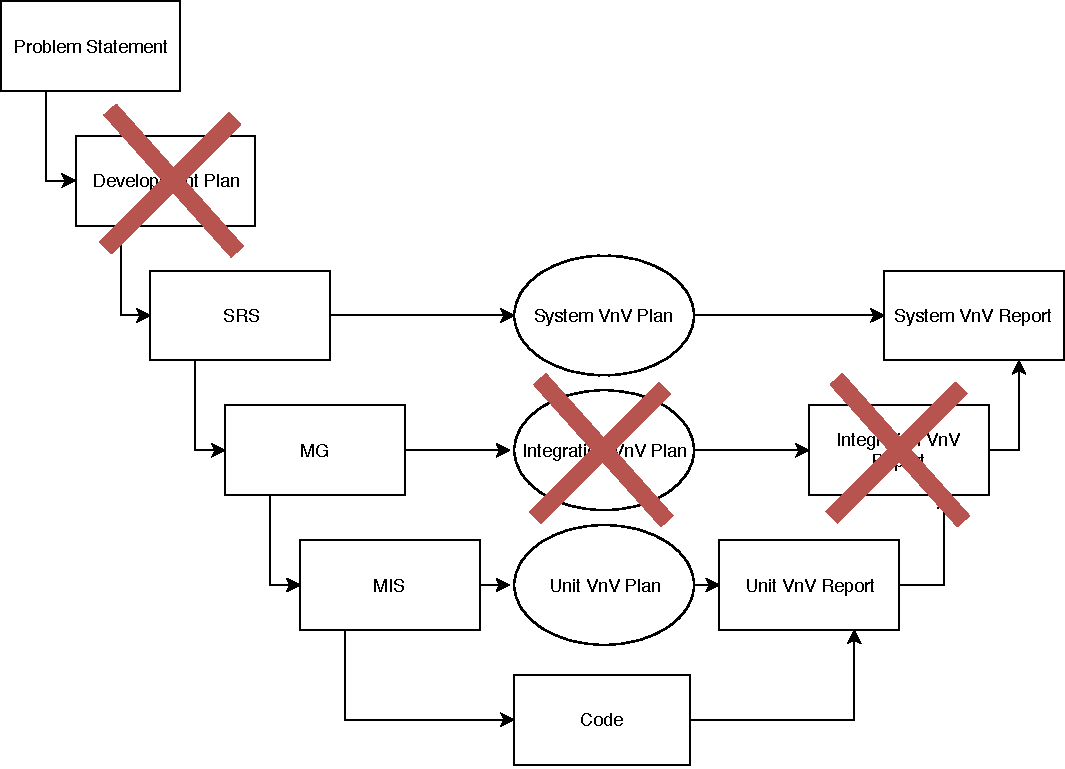
\includegraphics[scale=0.55]{../Figures/VModelOfProcessXOut.pdf}
\end{center}
\vspace{-1.0cm}

\end{frame}

%%%%%%%%%%%%%%%%%%%%%%%%%%%%%%%%%%%%%%

\begin{frame}
\frametitle{Administrative Details: Grade Assessment}

\begin {enumerate}

\item Presentations and class discussion 10\%

\item Quality of GitHub issues provided to classmates 5\%

\item Problem Statement 0\%

\item System Requirements Specification (SRS) 20\%

\item Verification and Validation (VnV) Plan 15\%
\begin{enumerate}
\item System VnV Plan 10\%
\item Unit VnV Plan 5\%
\end{enumerate}

\item Module Guide (MG) 5\%

\item Module Interface Specification (MIS) 15\%

\item Final Documentation 30\%
\begin{enumerate}
\item Problem Statement, SRS, System VnV Plan, MG, MIS, Unit VnV Plan (Revised)
\item Code
\item System VnV Report
\item Unit VnV Report
\end{enumerate}

\end {enumerate}

\end{frame}

%%%%%%%%%%%%%%%%%%%%%%%%%%%%%%%%%%%%%%%%%%%%%%%%%%

\begin{frame}
\frametitle{Administrative Details: Report Deadlines}
~\newline
\begin{tabular}{l l l}
Problem Statement & Week 02 & Sept 14\\
System Requirements Specification (SRS) & Week 05 & Oct 4\\
System VnV Plan & Week 07 & Oct 22\\
Module Guide (MG) & Week 09 & Nov 5\\
Module Interface Specification (MIS) & Week 11 & Nov 19\\
Unit VnV Plan & Week 13 & Dec 3\\
Final Documentation & Week 14 & Dec 10\\
\end {tabular}

\bi
\item The written deliverables will be graded based on the repo contents as of
11:59 pm of the due date
\item If you need an extension, please ask
\item Two days after each major deliverable, your GitHub issues will be due
\ei

\end{frame}

%%%%%%%%%%%%%%%%%%%%%%%%%%%%%%%%%%%%%%%%%%%%%%%%%%

\begin{frame}
\frametitle{Administrative Details: Presentations}

~\newline
\begin{tabular}{l l l}
SRS Present & Week 04 & Week of Sept 24\\
Syst.\ VnV Present & Week 06 & Week of Oct 15\\
MG Present & Week 08 & Week of Oct 29\\
MIS Present & Week 10 & Week of Nov 12\\
Unit VnV or Implement Present & Week 12 & Week of Nov 26\\
\end {tabular}

\bi
\item Tentative dates
\item Specific schedule depends on final class registration and need
\item Informal presentations with the goal of improving everyone's written
  deliverables
\item You will be assigned to ask questions of your colleagues
\ei

\end{frame}

%%%%%%%%%%%%%%%%%%%%%%%%%%%%%%%%%%%%%%%%%%%%%%%%%%

\begin{frame}
\frametitle{Introductions}

\begin{itemize}
\item Your name
\item Degree program
\item Academic background
\item Experience with:
\begin{itemize}
\item Scientific computing
\item Continuous math
\item Discrete math
\item Software engineering
\item Software development technology
\bi
\item Git
\item GitHub or GitLab
\item LaTeX
\item Make etc.
\ei
\end{itemize}
\item What do you hope to get out of this course?
\end{itemize}

\end{frame}

%%%%%%%%%%%%%%%%%%%%%%%%%%%%%%%%%%%%%%%%%%%%%%%%%%%%%%%%%%%%%%%%%%%%%%%%%%%%%

\begin{frame}
\frametitle{Project Selection: Desired Qualities}
\begin{itemize}
\item Related to scientific computing
\item Simple, but not trivial
\item If feasible, select a project related to your research
\item Ideally, re-implement existing software
\item Each student project needs to be unique
\item Possibly a specific physical problem
\item Possibly a (family of) general purpose tool(s)
\item Some examples follow, the links are just places to get started
\end{itemize}
\end{frame}

%%%%%%%%%%%%%%%%%%%%%%%%%%%%%%%%%%%%%%%%%%%%%%%%%%

\begin{frame}
\frametitle{Project Selection: Specific Physical Problem}
\begin{itemize}
\item
  \href{https://ocw.mit.edu/courses/mathematics/18-303-linear-partial-differential-equations-fall-2006/lecture-notes/heateqni.pdf}{
    Heated
    rod}
\item \href{http://www.tech.plym.ac.uk/sme/THER204B-web/Heatran2.PDF}{Heated plate}
\item \href{https://en.wikipedia.org/wiki/Double_pendulum}{Double pendulum}
\item \href{http://chrishecker.com/Rigid_Body_Dynamics}{Rigid body dynamics}
\item Column buckling
\item \href{https://en.wikipedia.org/wiki/Harmonic_oscillator}{Damped harmonic oscillator}
\item Stoichiometric calculations (chemical balance)
\item
  \href{http://www.tiem.utk.edu/~gross/bioed/bealsmodules/predator-prey.html}{Predator
    prey dynamics}
\item Imaging: filters, edge detection etc.
\item Medical Imaging
\item etc.
\end{itemize}

\end{frame}

%%%%%%%%%%%%%%%%%%%%%%%%%%%%%%%%%%%%%%%%%%%%%%%%%%

\begin{frame}
\frametitle{Project Selection: Family of General Purpose Tools}
\begin{itemize}
\item \href{https://en.wikipedia.org/wiki/Numerical_methods_for_ordinary_differential_equations}{Solution of ODEs}
\item \href{https://en.wikibooks.org/wiki/Numerical_Methods/Solution_of_Linear_Equation_Systems}{Solution of $A x = b$}
\item \href{https://en.wikipedia.org/wiki/Linear_regression}{Regression}
\item \href{https://en.wikibooks.org/wiki/Introduction_to_Numerical_Methods/Interpolation}{Interpolation}
\item \href{https://en.wikipedia.org/wiki/Numerical_integration}{Numerical integration}
\item \href{https://en.wikipedia.org/wiki/Fast_Fourier_transform}{FFT}
\item \href{https://en.wikipedia.org/wiki/Mesh_generation}{Mesh generation}
\item \href{https://en.wikipedia.org/wiki/Finite_element_method}{Finite element method}
\item Any chapter from a standard numerical methods textbook
\item etc.
\end{itemize}
\end{frame}

%%%%%%%%%%%%%%%%%%%%%%%%%%%%%%%%%%%%%%%%%%%%%%%%%%

\begin{frame}
\frametitle{Tool Tutorials}
\begin{itemize}
\item Best way to learn is by doing
\item Some getting started information and exercises in the ToolTutorials
  folder, modified from undergrad classes
\item Many other resources on-line
\item Your colleagues can help too
\end{itemize}
\end{frame}

%%%%%%%%%%%%%%%%%%%%%%%%%%%%%%%%%%%%%%%%%%%%%%%%%%

\begin{frame}
\frametitle{Git, GitLab and GitHub}
\begin{itemize}
\item Git manages changes to documents
\bi
\item Tracks changes
\item Keeps history, you can roll back
\item Useful documentation over time
\item Allows people to work simultaneously
\ei
\item Benefits for SC \cite{WilsonEtAl2016}
\bi
\item Not necessary to make a backup copy of everything, stores just enough
  information to recreate
\item Do not need to come up with names for backup copies - same file name, but
  with timestamps
\item Enforces changelog discipline
\item Facilitates identifying conflict and merging changes
\ei
\item The real bottleneck in scientific computing~\cite{Wilson2006}
\end{itemize}
\end{frame}

%%%%%%%%%%%%%%%%%%%%%%%%%%%%%%%%%%%%%%%%%%%%%%%%%%

\begin{frame}
\frametitle{Git Typical Usage}

First either init repo or clone (git init, git clone), then typical workflow is
\be
\item update repo (git pull)
\item create files
\item stage changes to be committed (git status, git add)
\item commit staged changes (git commit -m ``message'')
\item push to remote, if using one (git push)
\ee
\bi
\item Commit after every separate issue, and when need to stop working
\item Always include a meaningful and descriptive commit message for the log
\item If a push reveals conflicts, take appropriate action to merge
\ei
\end{frame}

%%%%%%%%%%%%%%%%%%%%%%%%%%%%%%%%%%%%%%%%%%%%%%%%%%

\begin{frame}
\frametitle{GitLab and GitHub Issue Tracking}

\bi
\item \href{https://gitlab.cas.mcmaster.ca/smiths/cas741/tree/master/ToolTutorials/gitAndGitLab}{See brief document in course repo}
\item \href{https://github.com/JacquesCarette/literate-scientific-software/issues}{See
  examples}
\item \href{https://gitlab.cas.mcmaster.ca/smiths/cas741/issues}{Create an issue}
\ei

\end{frame}

%%%%%%%%%%%%%%%%%%%%%%%%%%%%%%%%%%%%%%%%%%%%%%%%%%

\begin{frame}
\frametitle{LaTeX}
\begin{itemize}
\item A typesetting language
\item \href{https://gitlab.cas.mcmaster.ca/smiths/cas741/tree/master/ToolTutorials/LaTeX}{Some initial information in course repo}
\item Start from an example
\bi
\item The lectures notes
\item The Blank Project Template
\item The problem statement
\ei
\end{itemize}
\end{frame}

%%%%%%%%%%%%%%%%%%%%%%%%%%%%%%%%%%%%%%%%%%%%%%%%%%

\begin{frame}
\frametitle{Suggested Reading Questions?}

\begin {itemize}

\item
  \href{https://gitlab.cas.mcmaster.ca/smiths/cas741/blob/master/ReferenceMaterial/SoftEngForScienceBook.pdf}
  {Smith2016~\cite{Smith2016}}
\item
  \href{https://gitlab.cas.mcmaster.ca/smiths/cas741/blob/master/ReferenceMaterial/SmithLaiAndKhedri2007fulltext.pdf}
  {SmithEtAl2007~\cite{SmithEtAl2007}}
\item
  \href{https://gitlab.cas.mcmaster.ca/smiths/cas741/blob/master/ReferenceMaterial/ParnasAndClements1986.pdf}
  {{ParnasAndClements1986}~\cite{ParnasAndClements1986}}
\item \href{https://github.com/smiths/swhs}{Solar Water Heating System Example}

\end{itemize}

\end{frame}

%%%%%%%%%%%%%%%%%%%%%%%%%%%%%%%%%%%%%%%%%%%%%%%%%%

\begin{frame}
\frametitle{SE For SC Literature}

\begin {itemize}

\item CAS 741 process is document driven, adapted
from the waterfall model~\cite{GhezziEtAl2003, VanVliet2000}
\item Many say a document driven process is not used by, nor suitable for,
scientific software.
\bi
\item Scientific developers naturally use an agile
  philosophy~\cite{AckroydEtAl2008, CarverEtAl2007, EasterbrookAndJohns2009, Segal2005}, 
\item or an amethododical process~\cite{Kelly2013}
\item or a knowledge acquisition driven process~\cite{Kelly2015}.
\ei
\item Scientists do not view rigid, process-heavy approaches,
  favorably~\cite{CarverEtAl2007}
\item Reports for each stage of development are counterproductive~\cite[p.~373]{Roache1998}
\item Up-front requirements are
impossible~\cite{CarverEtAl2007, SegalAndMorris2008}
\item \structure{What are some arguments in favour of a rational document driven
    process?}
\end{itemize}

\end{frame}

%%%%%%%%%%%%%%%%%%%%%%%%%%%%%%%%%%%%%%%%%%%%%%%%%%

\begin{frame}
\frametitle{Counter Arguments}

\begin {itemize}

\item Just because document driven is not used, does not mean it will not work
\item Documentation provides many
benefits~\cite{Parnas2010}: 
\bi
\item easier reuse of old designs
\item better communication about requirements
\item more useful design reviews
\item easier integration of separately
written modules
\item more effective code inspection
\item more effective testing
\item more efficient corrections and improvements.
\ei
\item Actually faking a rational design process
\item Too complex for up-front requirements sounds like an excuse
\bi
\item Laws of physics/science slow to change
\item Often simple design patterns
\item Think program family, not individual member
\ei
\end{itemize}

\end{frame}

%%%%%%%%%%%%%%%%%%%%%%%%%%%%%%%%%%%%%%%%%%%%%%%%%%

\begin{frame}
\frametitle{Literature on SE applied to SCS}

\begin {itemize}

\item Highlights problems with SE
\begin{itemize}
\item
  \href{https://gitlab.cas.mcmaster.ca/smiths/cas741/blob/master/ReferenceMaterial/Miller2006.pdf}
  {Miller2006~\cite{Miller2006}}
\item
  \href{https://gitlab.cas.mcmaster.ca/smiths/cas741/blob/master/ReferenceMaterial/Hatton2007.pdf}
  {Hatton2007~\cite{Hatton2007}}
\item Sleipner A oil rig collapse~\cite[p.~38]{OliveiraAndStewart2006}
\item Patriot missile disaster~\cite[p.~36]{OliveiraAndStewart2006}
\end{itemize}
\item Highlights gap/chasm between SE and SC
\begin{itemize}
\item
  \href{https://gitlab.cas.mcmaster.ca/smiths/cas741/blob/master/ReferenceMaterial/Kelly2007.pdf}
  {Kelly2007~\cite{Kelly2007}}
\item
  \href{https://gitlab.cas.mcmaster.ca/smiths/cas741/blob/master/ReferenceMaterial/Storer2017.pdf}
  {Storer2017~\cite{Storer2017}}
\end{itemize}
\item Studies of SE applied to SC
\begin{itemize}
\item
  \href{https://gitlab.cas.mcmaster.ca/smiths/cas741/blob/master/ReferenceMaterial/CarverEtAl2007.pdf}
  {CarverEtAl2007~\cite{CarverEtAl2007}}
\item
  \href{https://gitlab.cas.mcmaster.ca/smiths/cas741/blob/master/ReferenceMaterial/Segal2005.pdf}
  {Segal2005~\cite{Segal2005}}
\end{itemize}

\end{itemize}

\end{frame}

%%%%%%%%%%%%%%%%%%%%%%%%%%%%%%%%%%%%%%%%%%%%%%%%%%

\begin{frame}
\frametitle{Literature on SE applied to SCS}

\begin {itemize}

\item Reproducibility
\begin{itemize}
\item
  \href{https://gitlab.cas.mcmaster.ca/smiths/cas741/blob/master/ReferenceMaterial/BaileyEtAl2016.pdf}
  {BaileyEtAl2016~\cite{BaileyEtAl2016}}
\item
  \href{https://gitlab.cas.mcmaster.ca/smiths/cas741/blob/master/ReferenceMaterial/BenureauAndRougier2017.pdf}
  {BenureauAndRougier2017~\cite{BenureauAndRougier2017}}
\end{itemize}

\item Future of SE for SC
\begin{itemize}
\item
  \href{https://gitlab.cas.mcmaster.ca/smiths/cas741/blob/master/ReferenceMaterial/JohansonAndHasselbring2018.pdf}
  {JohansonAndHasselbring2018~\cite{JohansonAndHasselbring2018}}
\item
  \href{https://gitlab.cas.mcmaster.ca/smiths/cas741/blob/master/ReferenceMaterial/Smith2018.pdf}
  {Smith2018~\cite{Smith2018}}
\end{itemize}

\end{itemize}

\end{frame}

%%%%%%%%%%%%%%%%%%%%%%%%%%%%%%%%%%%%%%%%%%%%%%%%%%

\begin{frame}[allowframebreaks]
\frametitle{References}

\bibliography{../../ReferenceMaterial/References}

\end{frame}

%%%%%%%%%%%%%%%%%%%%%%%%%%%%%%%%%%%%%%%%%%%%%%%%%%%%%%

\end{document}